\subsection{Topología ferroviaria original}

	El quinto ejemplo, ilustrado en la Figura \ref{fig:EJ5_1}, es una topología de dos vías principales paralelas y disconexas, con sus correspondientes desvíos para poder operar cada línea en ambos sentidos. La primera vía principal, la vía superior, utiliza los cambios de vías Sw01 y Sw02 para permitir circular dos formaciones en sentido contrario. En tanto que la segunda vía principal, la vía inferior, utiliza los cambios de vías Sw03 y Sw04 para el mismo fin. El objetivo de este ejemplo fue comprobar el funcionamiento del RNA con una topología de dos bypasses independientes y disconexos.
	
	\begin{figure}[h]
		\centering
		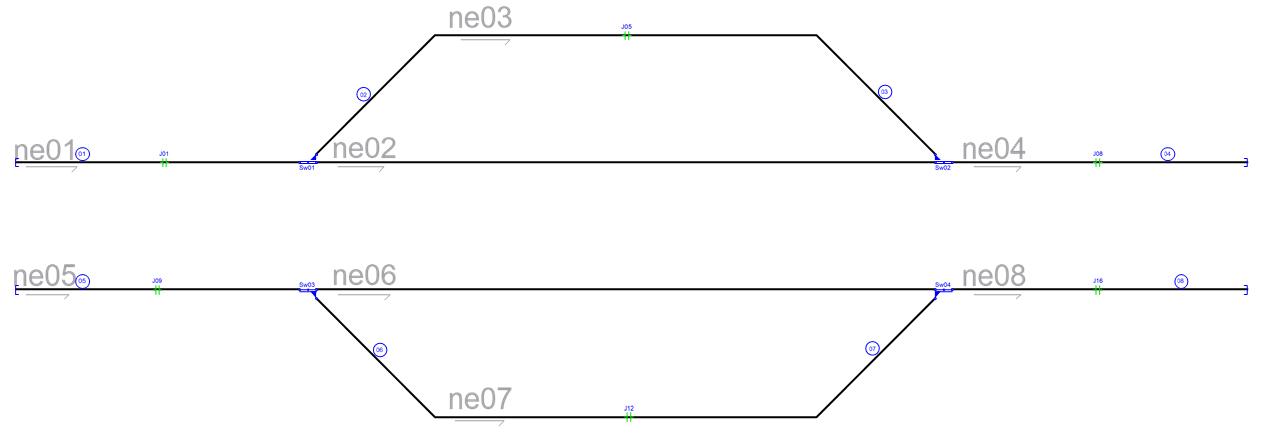
\includegraphics[width=1\textwidth]{resultados-obtenidos/ejemplo5/images/5_empty.png}
		\centering\caption{Topología ferroviaria del ejemplo 5 sin señalamiento.}
		\label{fig:EJ5_1}
	\end{figure}
	
	Para incrementar la dificultad del análisis y obtener resultados mas completos, todos los finales de vías absolutos. Además, se incluyeron junturas entre los finales de vías y los cambios de vías.
